\chapter{Anwendungsszenarien}
\section{Text-Mining, Natural Language Processing}
\section{Soziale Netze}
Unter dem Begriff Sozialem Netz versteht man eine Menge an Teilnehmern, häufig sind dies natürliche Personen, und verschiedenen Arten an Relationen zwischen diesen. Das durch die Beziehungen gebildete Netz lässt sich problemlos als Graph darstellen, indem die Teilnehmer als Knoten des Graphen dargestellt und die Beziehungen auf die Kanten abgebildet werden.

\begin{figure}
	\caption{Auschnitt aus Facebooks Socail-Graph: Checkin \cite{facebookTao}}
	\label{fig:fbCheckin}
	\centering
	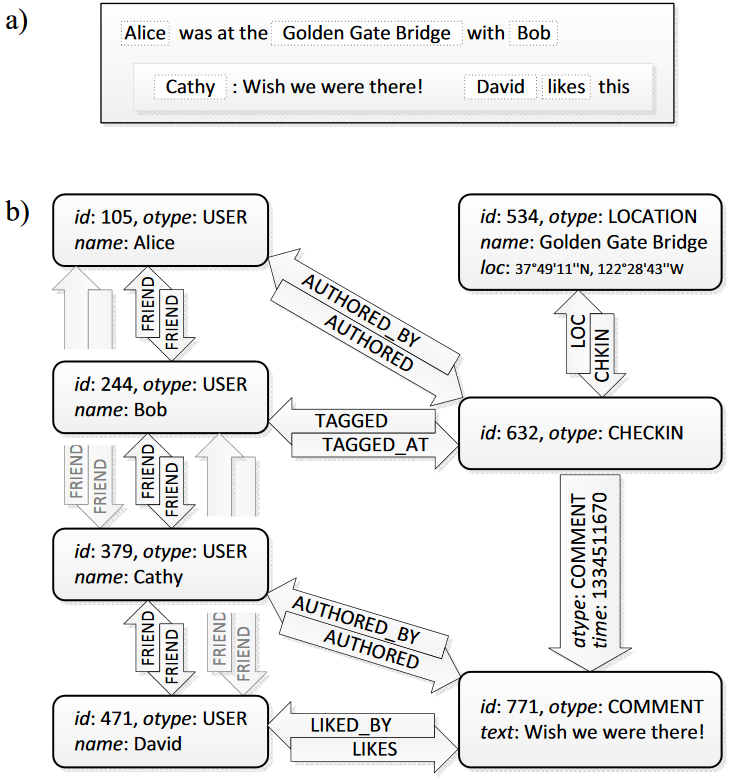
\includegraphics[width=0.7\textwidth]{images/facebook_checkin.png}
\end{figure}

Abbildung~\ref{fig:fbCheckin} zeigt beispielhaft wie ein Teil des Sozialen Netzes von Facebook aussieht. Anhand solcher Einträge wird für jeden einzelnen Nutzer eine personalisierte Startseite in Echtzeit erzeugt, dementsprechend wichtig ist ein performanter Datenzugriff. Um den Anforderungen gerecht zu werden hat Facebook eine eigene Graph-ähnliche API namens TAO entwickelt, welche den Datenbankzugriff effizient steuert. TAO stellt minimale Create/Update/Delete-Kommandos für Knoten und Kanten bereit. Der Großteil der Datenbankzugriffe ist allerdings lesend, folgende Querys sind möglich \cite{facebookTao}:
\begin{itemize}
	\item Alle Assoziation eines Typs zu einem Knoten
	\item Anzahl der Assoziationen eines Typs an einem Knoten
	\item Alle Nachbarn bis zur Tiefe n über eine bestimmte Assoziation
\end{itemize}
Dies ist ausreichend um mittels Verfahren wie Zentralitätsberechnung, Dichte und Cliquenanalyse für den Nutzer relevante Beiträge zu bestimmen \cite{sozialeNetzwerkanalyse}.

\section{Betrugserkennung}
\section{Empfehlungs-Engine}
\section{Verkehrsnetze}
\section{Stammdatenmanagement}
